\section{Pendahuluan}
Algoritma ElGamal, yang diperkenalkan oleh Taher ElGamal pada tahun 1985 \citep{elgamal1985}, adalah sistem kriptografi kunci-publik yang didasarkan pada kesulitan komputasi dari masalah logaritma diskrit dalam grup finit. Berbeda dengan RSA yang didasarkan pada pemfaktoran bilangan bulat besar, ElGamal lebih erat kaitannya dengan protokol pertukaran kunci Diffie-Hellman.

Perbandingan ringkas kedua algoritma disajikan pada Tabel~\ref{tab:elgamal-vs-rsa}.

\begin{table}[htbp]
    \centering
    \caption{Perbandingan algoritma ElGamal dan RSA}
    \label{tab:elgamal-vs-rsa}
    \begin{tabularx}{\linewidth}{|l|X|X|}
    \hline
    \textbf{Aspek} & \textbf{ElGamal} & \textbf{RSA} \\
    \hline
    Landasan keamanan & Masalah logaritma diskrit & Pemfaktoran bilangan bulat besar \\
    \hline
    Sifat enkripsi & Acak: cipherteks berbeda untuk plainteks yang sama & Deterministik \\
    \hline
    Ukuran cipherteks & Dua kali panjang plainteks & Sekitar panjang modulus \\
    \hline
    Skema tanda tangan & ElGamal dan DSA & RSA (PKCS\#1) \\
    \hline
    \end{tabularx}
\end{table}


\begin{figure}[htbp]
    \centering
    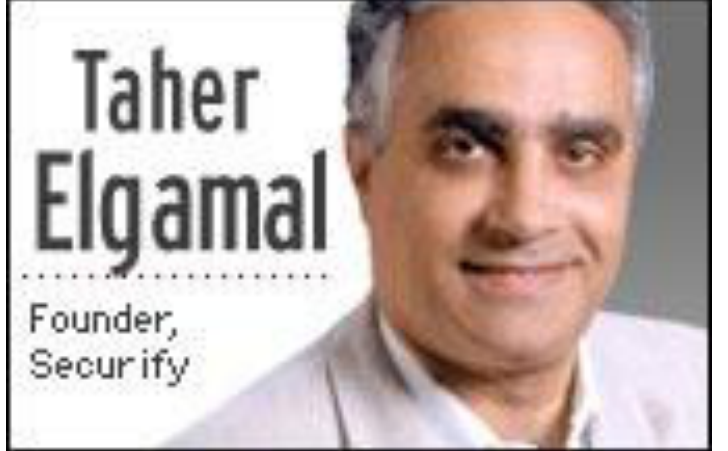
\includegraphics[width=0.42\linewidth, height=0.4\textheight, keepaspectratio]{figures/taher-elgamal.png}
    \caption{Taher Elgamal, perancang algoritma kriptografi kunci-publik ElGamal}
    \label{fig:taher-elgamal}
    \sumber{Munir, \textit{IF4020 Kriptografi}, ITB.}
\end{figure}
